\documentclass[11pt]{article}
\ifdefined\pdfinfoomitdate\pdfinfoomitdate=1\fi
\ifdefined\pdftrailerid\pdftrailerid{}\fi
\ifdefined\pdfsuppressptexinfo\pdfsuppressptexinfo=15\fi
\usepackage[T1]{fontenc}
\usepackage{lmodern}
\usepackage[margin=1.05in]{geometry}
\usepackage{amsmath,amssymb,amsthm,mathtools}
\usepackage{microtype}
\usepackage{enumitem}
\usepackage{xurl}
\usepackage{tikz}
\usepackage[hidelinks]{hyperref}
\usepackage[nameinlink,noabbrev,capitalise]{cleveref}
\setlist[itemize]{topsep=4pt,itemsep=2pt,parsep=0pt}
\setlist[enumerate]{topsep=4pt,itemsep=2pt,parsep=0pt}
\numberwithin{equation}{section}
\newtheorem{theorem}{Theorem}[section]
\newtheorem{lemma}[theorem]{Lemma}
\newtheorem{proposition}[theorem]{Proposition}
\newtheorem{corollary}[theorem]{Corollary}
\theoremstyle{definition}
\newtheorem{definition}[theorem]{Definition}
\theoremstyle{remark}
\newtheorem{remark}[theorem]{Remark}
\crefname{theorem}{Theorem}{Theorems}
\crefname{lemma}{Lemma}{Lemmas}
\crefname{proposition}{Proposition}{Propositions}
\crefname{corollary}{Corollary}{Corollaries}
\crefname{definition}{Definition}{Definitions}
\crefname{remark}{Remark}{Remarks}
\newcommand{\R}{\mathbb R}
\newcommand{\N}{\mathbb N}
\newcommand{\F}{\mathcal F}
\newcommand{\Lip}{\operatorname{Lip}}
\newcommand{\Lipnorm}[1]{\|#1\|_{\mathrm{Lip}}}
\newcommand{\TV}{\mathrm{TV}}
\newcommand{\norm}[1]{\left\|#1\right\|}
\newcommand{\abs}[1]{\left|#1\right|}
\newcommand{\dist}{\operatorname{dist}}
\newcommand{\E}{\mathbb E}
\newcommand{\Pp}{\mathbb P}
\newcommand{\Id}{\operatorname{Id}}
\DeclareMathOperator{\supp}{supp}
\hypersetup{
  pdftitle={A uniformly discrete counterexample to bounded approximation in Lipschitz-free spaces},
  pdfauthor={OpenAI},
  pdfsubject={A countable uniformly discrete metric space whose real Lipschitz-free space has AP but fails BAP}
}

\title{A uniformly discrete counterexample to bounded approximation in Lipschitz-free spaces}
\author{OpenAI}
\date{September 26, 2026}
\begin{document}
\maketitle
\begin{abstract}
We construct a countable uniformly discrete metric space whose real
Lipschitz-free space has the approximation property but fails the
bounded approximation property, answering Kalton's question negatively.
The identity can be approximated on every compact set by finite-rank
operators, but no uniform bound on their norms is possible.
\end{abstract}
\section{Introduction}\label{sec:introduction}

Uniform discreteness keeps distinct points of a metric space a fixed positive
distance apart. For its Lipschitz-free space, this separation guarantees the
approximation property: the identity can be approximated on each compact set
by finite-rank operators. Kalton asked whether the approximating operators
can always be chosen with one bound on their norms
\cite[Proposition~4.4 and following remarks, p.~185]{Kalton04}. The question
was restated by Godefroy and Ozawa \cite[Question~1]{GodefroyOzawa14} and in
Godefroy's survey \cite[Problem~6.2]{Godefroy15}. We construct a countable
uniformly discrete space for which no such bound exists.

We work over the real scalars. For a pointed metric space $(M,d,o)$, let
$\Lip_0(M)$ be the Banach space of real Lipschitz functions vanishing at $o$,
with the Lipschitz constant as norm. Its \emph{Lipschitz-free space} is
\[
 \F(M)=\overline{\operatorname{span}}\{\delta_x:x\in M\}
 \subseteq\Lip_0(M)^*,\qquad \delta_x(f)=f(x).
\]
Thus $\delta_o=0$ and $\norm{\delta_x-\delta_y}=d(x,y)$. The latter
identity follows from the Lipschitz inequality and the test function
$z\mapsto d(z,y)-d(o,y)$.
The construction originates in the molecular spaces of Arens and Eells
\cite[\S2]{ArensEells56}; its linearization properties and complemented free
subspaces are central to the work of Godefroy and Kalton
\cite[\S2]{GodefroyKalton03}.

A Banach space $X$ has the \emph{approximation property} (AP) if for every
norm-compact set $C\subseteq X$ and every $\varepsilon>0$ there is a bounded
finite-rank linear operator $T:X\to X$ with
$\sup_{u\in C}\norm{Tu-u}<\varepsilon$. For $\lambda\ge1$, it has
$\lambda$-BAP if these operators can always be chosen with
$\norm{T}\le\lambda$. The bounded approximation property (BAP) means
$\lambda$-BAP for some finite $\lambda$, and the metric approximation
property (MAP) means $1$-BAP. In AP the norm may depend on $C$ and
$\varepsilon$; in BAP one bound must work for all of them. A metric space
is \emph{proper} if its closed bounded balls are compact.

\begin{theorem}\label{thm:main}
There is a countable, unbounded, nonproper pointed metric space $(M,d,o)$
such that $d(x,y)\ge1$ for distinct points and $\F(M)$ has AP but fails
$\lambda$-BAP for every finite $\lambda\ge1$.
\end{theorem}

The distinction between discrete and uniformly discrete matters here.
Smith gives countable complete discrete spaces whose free spaces have AP
and fail BAP, without asserting a common positive lower bound on all
nonzero distances \cite[Theorem~1.3 and the surrounding discussion]{Smith26}.
\Cref{thm:main}
supplies that lower bound. The example is necessarily outside the countable
proper case: Dalet proved MAP for free spaces over countable proper metric
spaces \cite[Theorem~2.6]{Dalet15}. Our example contains an infinite separated
subset in a bounded ball.
Uniform discreteness also imposes strong sequential structure: C\'uth and
Kalenda prove a quantitative strengthening of the Schur property for these
free spaces \cite[Theorem~1.1]{CuthKalenda26}, so weakly convergent sequences
converge in norm. Their April 2026 introduction still records the BAP
question addressed here.

The same example has a nonlinear consequence. Kalton asked whether every
separable Banach space is \emph{approximable} \cite[Problem~1, p.~1260]{Kalton12}.
For such a space $X$, this means that there is an equi-uniformly continuous
sequence of maps $\psi_n:X\to X$, each with relatively compact range, such
that $\psi_n(x)\to x$ for every $x\in X$. Equi-uniform continuity means that
the choice of $\delta$ for a given $\varepsilon$ in the uniform-continuity
condition works for every $\psi_n$. The space $X=\F(M)$ in \Cref{thm:main}
is not approximable, although it has AP. \Cref{sec:nonlinear} explains the
short implication from Kalton's net theorem that gives this consequence.

\subsection{A finite obstruction in each bounded block}

The main construction concerns a prescribed operator norm bound $p$.
It produces a bounded metric space and a finite set of points, called
anchors, at which every finite-rank operator of norm at most $p$ makes a
definite error. The distinction from earlier finite extension obstructions
is important. For a finite pointed metric pair $A\subseteq N$ containing
the basepoint, a linear extension operator
$E:\Lip_0(A)\to\Lip_0(N)$ must satisfy $(Ef)|_A=f$ for every $f$.
Brudnyi and Brudnyi give finite subsets of integer $\ell_1$ cubes for which
the least possible norm of an exact linear extension operator grows without bound
\cite[preprint Lemma~10.5, pp.~46--47]{BrudnyiBrudnyi07}. Godefroy and Ozawa
\cite[Proposition~7]{GodefroyOzawa14} obtain arbitrarily large lower bounds for
finite metric pairs from a compact free space failing AP. By
finite-dimensional duality, an extension operator corresponds, with the
same norm, to a projection from $\F(N)$ onto the span of the evaluations
from $A$. These bounds therefore concern projections with a prescribed
range. On the finite-dimensional space $\F(N)$, the identity remains a
finite-rank operator of norm at most one. Our block is infinite, and its
fixed finite anchor set obstructs approximation by every operator of norm
at most $p$ whose range is finite-dimensional.

\begin{theorem}\label{thm:blocks}
For each integer $p\ge1$, there are a bounded countably infinite pointed
metric space $(M_p,d_p,o)$ and a finite set $A_p\subseteq M_p$ containing
$o$ such that
\[
 d_p(x,y)\ge1\quad(x\ne y),\qquad
 \operatorname{diam}M_p\le B_p:=300p^2+150p+5,
\]
and every bounded finite-rank linear operator
$T_0:\F(M_p)\to\F(M_p)$ with $\norm{T_0}\le p$ satisfies
\[
 \max_{a\in A_p}\norm{T_0\delta_a-\delta_a}\ge\frac12.
\]
\end{theorem}

Each individual block nevertheless has BAP. The coefficient identification
for bounded uniformly discrete spaces appears in
\cite[Theorem~4.14]{AACD20}, with the bounds used here in
\cite[Lemma~3.4]{CuthKalenda26}. Our proof in \Cref{prop:coefficients} identifies $\F(M_p)$ with
$\ell_1(M_p\setminus\{o\})$, and coordinate truncations give
$2B_p$-BAP alongside the obstruction at $p$. Transporting the free-space
norm to real $\ell_1$ gives the following quantitative consequence. It
also answers a separate question: does every equivalent norm on real
$\ell_1$ have MAP? Kalton observed that a positive answer would imply BAP
for every uniformly discrete free space \cite[p.~1260]{Kalton12}. The case
$p=1$ below gives a direct negative answer.

\begin{corollary}\label{cor:renorming}
For each integer $p\ge1$, real $\ell_1$ has an equivalent norm
$\norm{\cdot}_p$ such that
\[
 \tfrac12\norm{c}_1\le\norm{c}_p\le B_p\norm{c}_1,
\]
and $(\ell_1,\norm{\cdot}_p)$ has $2B_p$-BAP but fails $p$-BAP.
For $p=1$, this norm fails MAP.
\end{corollary}

To pass from the blocks to \Cref{thm:main}, identify their
basepoints and put
\[
 d(x,y)=d_p(x,o)+d_q(y,o)
 \quad\text{if }x\in M_p\setminus\{o\},\ y\in M_q\setminus\{o\},\ p\ne q.
\]
Each block then has a pointed $1$-Lipschitz retraction from the resulting
metric wedge. On free spaces, inclusion and retraction induce contractions
whose composite is the identity. Thus a BAP bound for the wedge would be
a bound for every block, contradicting \Cref{thm:blocks}.

The same decomposition proves AP directly. First retain finitely many
blocks by a contractive projection that approximates the chosen compact
set. Then approximate its images in those blocks, using their individual
BAPs. Only finitely many operator norms occur at this stage, so the
resulting operator is bounded. The bound is allowed to grow as more
blocks are retained.

\subsection{The obstruction: signed measures and opposing tests}

The block itself consists of two kinds of points: vertices of finite source
graphs and anchors that join those graphs into a bounded metric space.
After a finite-rank operator is given, we choose a finite subset $S$ of
these same points to support the range of a nearby operator. Thus $S$ may
contain source vertices or anchors and may depend on the operator.

The source graphs have a fixed large degree. For every fixed radius, the
frequencies of their colored neighborhoods approach the corresponding
probabilities in a regular tree of that degree with independent uniform
vertex colors. A vertex is labeled by its
capped distances to the color classes. These labels vary by at most one
across an edge, and each label has only a bounded number of coordinates
below the cap. Vertices with the same label attach to the same anchor
by a long edge. There are only finitely many possible labels, hence
finitely many anchors. Joining the anchors makes the whole block bounded,
while sufficiently small metric balls remain inside a single source
graph and contain a uniformly bounded number of points.

Suppose a finite-rank operator of small norm approximates the
anchor evaluations. An arbitrarily small perturbation gives an operator
$T$ with $\norm{T}\le2p$ whose range has a common finite support
$S\subset M_p$. Adding a coefficient at the
basepoint allows us to write its values as signed measures $\mu_x$ on
$S$, each of mass one and uniformly bounded total variation. For the
height $L=10p$, a nonnegative bump $b_x:M_p\to[0,L]$ detects support points
whose labels are close to the label of $x$. It takes its maximum $L$ at the
anchor $a(x)$ attached to $x$ and has a small Lipschitz constant, in
particular at most one. The operator norm controls the comparison from
$x$ to $a(x)$, while the anchor approximation controls the value there.
The small slope of $b_x$ makes their combined loss from the anchor value
at most $L/4$. The affine representation therefore gives
\[
 (T\delta_x)(b_x-b_x(o))+b_x(o)=\int b_x\,d\mu_x\ge\frac{3L}{4}.
\]
No positivity of $\mu_x$ is assumed.

A source walk is \emph{nonbacktracking} if it never immediately reverses
an edge incidence. The color structure makes it rare for a source vertex
to start a long nonbacktracking walk that can be tracked by nearby support
points with compatible labels. Such a walk is \emph{matched} if one can
choose a support point at each step with a compatible label, while
consecutive support points stay within distance $2L$. For a prescribed
support point, compatibility allows only a
small set of source colors. A bound on small metric balls limits the
possible next support points. On the limiting tree, the source colors
along a nonbacktracking walk are independent. Choosing many colors
therefore makes long matched walks rare.

Call a vertex \emph{good} if no matched walk of the chosen long length
starts there, and \emph{bad} otherwise. At a good vertex, record the longest matched walk
beginning in each outgoing direction, for each fixed
initial support point. Declare a direction exceptional only when its
record is strictly larger than every other record. There is at most
one such direction per support point. If nearby support points match
the two ends of an edge whose endpoints are good, at least one of the two directions along that
edge must be exceptional: otherwise prepending the edge to a longest
walk in another direction would force each of two finite records to be
larger than the other.

For an oriented incidence $e:x\to y$, let $E_e$ be the support points for
which $e$ is exceptional at $x$; at a bad vertex we put every support point
in $E_e$. We prescribe $b_x$ on $S\setminus E_e$ and $-b_y$ on
$S\setminus E_{\bar e}$, where $\bar e$ is the reverse incidence. Within
each set the prescribed values satisfy the Lipschitz inequality because
the bumps do. For a cross pair $j\in S\setminus E_e$ and
$j'\in S\setminus E_{\bar e}$, the record argument shows that if
$d_p(j,j')<2L$, then both $b_x(j)$ and $b_y(j')$ vanish. If the distance
is at least $2L$, their sum is bounded by that distance. Thus all the
prescribed values together are $1$-Lipschitz. Scalar extension followed by
clipping gives a $1$-Lipschitz test $f_e:M_p\to[-L,L]$. Its pairing satisfies
\[
 \int f_e\,d(\mu_x-\mu_y)
 \ge \frac{3L}{2}
 -2L\bigl(|\mu_x|(E_e)+|\mu_y|(E_{\bar e})\bigr).
\]
Here $|\mu_x|(E_e)$ is the sum of the absolute values of the coefficients
of $\mu_x$ on $E_e$. Each support point belongs to at most one exceptional
set at a good vertex. Averaging over all oriented incidences therefore
divides the corresponding variation loss by the graph degree; the small
fraction of bad vertices controls the remaining loss. Since source-edge
endpoints have $d_p$-distance at most one, the affine pairing bounds each
test pairing in absolute value by $\norm{T}\le2p$. The averaged lower bound
contradicts this upper bound.

The order of choices is essential. The entire deterministic graph
sequence, metric block, and anchors are fixed before the operator and
its support $S$. We then choose the walk length and one sufficiently
large source graph. Local convergence applies to every finite colored
event, including the event specified by this already fixed support.
There is no assumption that the operator was chosen independently of
the graph sequence.

\subsection{Methods and organization}

For the graph construction we use the independent-permutation model
described by Friedman \cite{Friedman04} and prove the local convergence
we need directly. The empirical rooted-neighborhood viewpoint is that
of Benjamini and Schramm \cite{BenjaminiSchramm01}. The scalar extension
step is an instance of McShane's classical extension principle
\cite{McShane34}; we give the needed formula for finite data and its proof.
A related comparison of nonbacktracking continuation lengths is used to
select parent directions in the graph algorithm of Ben-David, Childs,
Gily\'en, Kretschmer, Podder, and Wang
\cite[\S6.1.2]{BenDavidEtAl24}. Our continuation records also depend on
the support state and are used to construct the scalar tests.

\Cref{sec:reduction} proves the coefficient estimate, the renorming
corollary, and the wedge reduction, assuming \Cref{thm:blocks}, and derives
the nonlinear consequence from Kalton's theorem.
\Cref{sec:blocks} constructs the colored graphs and bounded block.
\Cref{sec:operators,sec:walks,sec:tests} prove \Cref{thm:blocks}:
they pass from an arbitrary finite-rank operator to signed measures,
bound matched walks, and derive the contradiction by scalar tests and
incidence averaging.

\section{From bounded blocks to AP without BAP}\label{sec:reduction}

The following sections will construct the blocks of \Cref{thm:blocks}.
Here we assume that theorem, prove the renorming and wedge results, and
derive the nonlinear consequence from Kalton's theorem. A bounded space with separation at least one has a
coefficient description by $\ell_1$, with an approximation bound
controlled by its diameter.
Joining the blocks preserves each of their obstructions, while retractions
onto finitely many blocks provide the approximations required for AP.

\subsection{The coefficient estimate}

The coefficient identification below appears in
\cite[Theorem~4.14]{AACD20}; the coefficient bounds are stated in
\cite[Lemma~3.4]{CuthKalenda26}. We include the proof and derive the
stated approximation bound from coordinate truncations.

\begin{proposition}\label{prop:coefficients}
Let $(N,d,o)$ be a countable pointed metric space such that
$d(x,y)\ge1$ for distinct points and $\operatorname{diam}N\le B<\infty$.
The map
\[
 J:\ell_1(N\setminus\{o\})\longrightarrow\F(N),
 \qquad Jc=\sum_{x\ne o}c_x\delta_x,
\]
is a linear isomorphism onto $\F(N)$ and satisfies
\begin{equation}\label{eq:coefficient-bounds}
 \tfrac12\norm{c}_1\le\norm{Jc}\le B\norm{c}_1.
\end{equation}
If $N\ne\{o\}$, then $\F(N)$ has $2B$-BAP. If $N=\{o\}$, both
spaces are zero.
\end{proposition}

\begin{proof}
First let $c$ be finitely supported. Since $\norm{\delta_x}=d(x,o)\le B$,
the triangle inequality gives the upper estimate in
\eqref{eq:coefficient-bounds}. For the lower estimate, define
$f_c:N\to\R$ to be $\operatorname{sign}(c_x)/2$ at each nonbasepoint
in the support of $c$, and zero elsewhere. This function vanishes at
$o$. Its values differ by at most one, so the separation assumption
makes it $1$-Lipschitz. Testing the evaluation combination against $f_c$
gives
\[
 \norm{Jc}\ge (Jc)(f_c)=\tfrac12\sum_{x\ne o}|c_x|.
\]

The upper estimate makes the series defining $Jc$ converge in $\F(N)$
for every $c\in\ell_1(N\setminus\{o\})$. Both estimates pass to this
extension by approximation with finitely supported families. In particular,
$J$ is injective and its inverse on its range has norm at most two.
The range is closed: if $Jc_m$ converges, then
\[
 \norm{c_m-c_j}_1\le2\norm{Jc_m-Jc_j}
\]
makes $(c_m)$ Cauchy, and continuity of $J$ identifies the limit of
$(Jc_m)$ as the image of the limit of $(c_m)$. The range also contains
every evaluation $\delta_x$, whose span is dense in $\F(N)$. It is
therefore all of $\F(N)$.

Suppose now that $N\ne\{o\}$; then $B\ge1$. Choose increasing finite
sets $E_m$ exhausting $N\setminus\{o\}$, and let $q_m$ be the associated
coordinate projections on $\ell_1(N\setminus\{o\})$. The operators
\[
 S_m=Jq_mJ^{-1}:\F(N)\longrightarrow\F(N)
\]
have finite rank and norm at most $B\cdot1\cdot2=2B$. Since
$q_mc\to c$ in $\ell_1$, they satisfy $S_mu\to u$ for every
$u\in\F(N)$. This convergence is uniform on compact sets. Indeed, for
a nonempty compact $C\subseteq\F(N)$ and $\varepsilon>0$, choose a
finite $\varepsilon/[3(2B+1)]$-net in $C$. For all sufficiently large
$m$, the error $\norm{S_mu-u}$ is less than $\varepsilon/3$ at every
point of the net. Since $\norm{S_m-\Id}\le2B+1$, the error at any
point of $C$ is then less than $2\varepsilon/3$, hence less than
$\varepsilon$. The empty compact set imposes no condition. If $N$ is
finite, the sequence of coordinate projections is eventually the identity.
This proves $2B$-BAP. The assertion for $N=\{o\}$ is immediate.
\end{proof}

\begin{proof}[Proof of \Cref{cor:renorming}]
Fix $p\ge1$. By \Cref{thm:blocks}, the set $M_p\setminus\{o\}$ is
countably infinite, so an enumeration identifies its coefficient space
with real $\ell_1$. Apply \Cref{prop:coefficients} with $B=B_p$, denote
its coefficient map by $J_p$, and define
$\norm{c}_p=\norm{J_pc}_{\F(M_p)}$. Equation
\eqref{eq:coefficient-bounds} gives the stated norm inequalities and
shows that this is an equivalent norm. For this norm, $J_p$ is a
surjective isometry. Conjugation by $J_p$ preserves operator norms,
finite rank, and approximation errors on corresponding compact sets.
It therefore transfers $2B_p$-BAP to the new norm, with
$2B_p=600p^2+300p+10$. If the new norm had $p$-BAP, the same conjugation
would give $p$-BAP on $\F(M_p)$. Applying it with accuracy $1/2$ to
the finite set $\{\delta_a:a\in A_p\}$ would contradict
\Cref{thm:blocks}. For $p=1$, this is precisely failure of MAP.
\end{proof}

\subsection{The metric wedge and its retractions}

Take disjoint copies of the spaces $M_p$ and identify only their
basepoints. Thus, as a set,
\[
 M=\{o\}\cup\bigsqcup_{p\ge1}(M_p\setminus\{o\}).
\]
Keep the distance $d_p$ within each block, and for nonbasepoint points
in distinct blocks set
\begin{equation}\label{eq:wedge-metric}
 d(x,y)=d_p(x,o)+d_q(y,o)
 \qquad(x\in M_p\setminus\{o\},\ y\in M_q\setminus\{o\},\ p\ne q).
\end{equation}
These rules define a metric. Symmetry and positivity are immediate.
For the triangle inequality, if the endpoints lie in one block, a
detour through a point $z$ in another block has length
$d_p(x,o)+2d_q(z,o)+d_p(y,o)\ge d_p(x,y)$. If the endpoints lie in
different blocks and the third point lies in one of those blocks, that
block's triangle inequality gives the required bound. A third point in
a third block adds twice its distance to $o$, and a third point equal
to $o$ gives equality. The remaining case is the triangle inequality
within a single block.

The space $M$ is countable. Within a block, distinct points remain at
distance at least one; in distinct blocks, nonbasepoint points are at
distance at least two. It is also unbounded. To see this using only
\Cref{thm:blocks}, suppose that $M$ had finite diameter $C_0$. Then
$C_0\ge1$, and every $M_p$ would have diameter at most $C_0$.
\Cref{prop:coefficients} would give $2C_0$-BAP on every $\F(M_p)$.
Choose an integer $p\ge\max\{1,2C_0\}$. Applying that property to
$\{\delta_a:a\in A_p\}$ with accuracy $1/2$ would produce a finite-rank
operator of norm at most $2C_0\le p$ whose error is less than $1/2$
at every anchor, contrary to \Cref{thm:blocks}.

Finally, the closed ball about $o$ of radius $B_1$ contains the
countably infinite $1$-separated set $M_1$. If this ball were compact,
its cover by open balls of radius $1/3$ would admit a finite subcover.
Each such ball contains at most one point of $M_1$, which is impossible.
Thus $M$ is nonproper.

For each $p$, let $i_p:M_p\to M$ be inclusion and let $r_p:M\to M_p$
fix $M_p$ and send all other blocks to $o$. Both are pointed
$1$-Lipschitz maps. Inclusion preserves distances. For the retraction,
the only case that needs an inequality has $x\in M_p$ and
$y\in M_q\setminus\{o\}$ for $q\ne p$; then
\[
 d_p(r_p(x),r_p(y))=d_p(x,o)\le d(x,y).
\]
If both points are outside $M_p$, their images coincide, and if both
are in $M_p$, their distance is preserved.

We use the elementary linearization property of free spaces; its role
in Banach-space geometry is developed in \cite[\S2]{GodefroyKalton03}.
If $u:N\to N'$ is pointed and $1$-Lipschitz, define on finite evaluation
combinations
\[
 \widehat u\left(\sum_x c_x\delta_x\right)=\sum_x c_x\delta_{u(x)}.
\]
Pullback of pointed scalar tests gives
\begin{align*}
 \left\|\sum_x c_x\delta_{u(x)}\right\|
 &=\sup_{\substack{f\in\Lip_0(N')\\\Lipnorm{f}\le1}}
       \left|\sum_x c_x(f\circ u)(x)\right|\\
 &\le\left\|\sum_x c_x\delta_x\right\|.
\end{align*}
This inequality makes the definition independent of the representation
of the evaluation combination, and it gives a unique continuous linear
extension $\widehat u:\F(N)\to\F(N')$ of norm at most one.
Applying it to $i_p$ and $r_p$ gives contractions
\[
 I_p:\F(M_p)\longrightarrow\F(M),\qquad
 P_p:\F(M)\longrightarrow\F(M_p).
\]
Their composite $P_pI_p$ fixes every evaluation, so it is the identity
on $\F(M_p)$. In particular, for every $v\in\F(M_p)$,
\[
 \norm{v}=\norm{P_pI_pv}\le\norm{I_pv}\le\norm{v};
\]
thus $I_p$ is an isometry.

\subsection{The approximation properties of the wedge}

Suppose that $\F(M)$ had $\lambda$-BAP for some finite $\lambda\ge1$.
Choose an integer $p\ge\lambda$ and apply that property with accuracy
$1/2$ to the finite, hence compact, set
$\{I_p\delta_a:a\in A_p\}$. Let $U$ be the resulting operator.
The compression $P_pUI_p$ has finite rank and norm at most
$\lambda\le p$, while for every $a\in A_p$,
\[
 \norm{P_pUI_p\delta_a-\delta_a}
 \le\norm{UI_p\delta_a-I_p\delta_a}<\tfrac12.
\]
This contradicts \Cref{thm:blocks}. All blocks and their anchor sets
were fixed before $\lambda$ and $U$ were chosen.

It remains to prove AP. Kalton's general theorem
\cite[Proposition~4.4]{Kalton04} gives AP for free spaces over uniformly
discrete metric spaces; the wedge structure provides a direct proof here.
For $N\ge1$, define
$r_{\le N}:M\to M$ to retain the first $N$ blocks and send every other
block to $o$. It is pointed and $1$-Lipschitz: distances in the retained
part are unchanged, distances in the collapsed part become zero, and
\eqref{eq:wedge-metric} bounds the image distance for a retained point
and a collapsed point. Its linearization is a contractive projection
\begin{equation}\label{eq:finite-block-projection}
 R_N=\sum_{p=1}^N I_pP_p.
\end{equation}
The equality follows on each evaluation $\delta_x$: the sum retains it
when $x$ is in one of the first $N$ blocks and sends it to zero otherwise.
The same check gives $R_N^2=R_N$. Continuity gives both identities on
$\F(M)$.

Every finite linear combination of evaluations is fixed by $R_N$ for
all sufficiently large $N$. These combinations are dense, and
$\norm{\Id-R_N}\le2$. Thus $R_Nu\to u$ for every $u\in\F(M)$:
given a finite evaluation combination $v$ fixed by $R_N$, one has
$\norm{R_Nu-u}\le2\norm{u-v}$. The finite-net argument in the proof of
\Cref{prop:coefficients}, applied now with $\norm{\Id-R_N}\le2$, makes
this convergence uniform on every norm-compact set.

Now fix a nonempty norm-compact $C\subseteq\F(M)$ and
$\varepsilon>0$. First choose $N\ge1$ such that
\[
 \sup_{u\in C}\norm{R_Nu-u}<\varepsilon/2.
\]
For each $1\le p\le N$, the image $P_p(C)$ is compact. By
\Cref{prop:coefficients}, choose a finite-rank operator
$T_p:\F(M_p)\to\F(M_p)$ with $\norm{T_p}\le2B_p$ and
\[
 \sup_{u\in C}\norm{T_pP_pu-P_pu}<\frac{\varepsilon}{2N}.
\]
The operator
\[
 T=\sum_{p=1}^N I_pT_pP_p:\F(M)\longrightarrow\F(M)
\]
has finite rank and is bounded, with
$\norm{T}\le\sum_{p=1}^N2B_p<\infty$. By
\eqref{eq:finite-block-projection}, for every $u\in C$,
\[
 \norm{Tu-u}
 \le\norm{R_Nu-u}
       +\sum_{p=1}^N\norm{T_pP_pu-P_pu}<\varepsilon.
\]
We first chose $N$ so that the contractive projection $R_N$ approximated
the whole compact set, and then chose the finitely many block operators.
Their combined norm may depend on $C$ and
$\varepsilon$, as AP permits. This proves AP, and the metric properties
and the preceding obstruction prove \Cref{thm:main} under
\Cref{thm:blocks}.

\subsection{Failure of nonlinear approximability}\label{sec:nonlinear}

We verify the nonlinear consequence stated in the introduction using
Kalton's characterization by nets \cite[Theorem~4.4 and p.~1260]{Kalton12}.
Let $X=\F(M)$ for the
wedge just constructed. It is separable because $M$ is countable, and
$\{\delta_x:x\in M\}$ is $1$-separated in $X$. Extend this set to a maximal
$1$-separated set $N_X\subseteq X$. Every point of $X$ is then within
distance one of $N_X$, so $N_X$ is a net: a separated set within a fixed
distance of every point of $X$. If $X$ were approximable, Kalton's theorem
would give one Lipschitz bound $\Lambda\ge1$ for maps $g:N_X\to N_X$
with relatively compact range that approximate any prescribed finite subset
as closely as desired. Separation makes each such range finite and turns
approximation within distance less than one into exact fixing. For a finite
$F\subseteq M$ containing $o$, choose $g$ fixing every $\delta_x$ with
$x\in F$. The restriction $x\mapsto g(\delta_x)$ is then a pointed
$\Lambda$-Lipschitz map from $M$ into $X$. The Banach-valued linearization
property of free spaces \cite[Lemma~3.2]{Kalton04} gives a finite-rank
operator $T_F:X\to X$ of norm at most $\Lambda$ satisfying
$T_F\delta_x=g(\delta_x)$ for all $x\in M$. To approximate a compact set,
approximate a finite net in it by finite evaluation combinations and put
all their supports in $F$. The operator $T_F$ fixes those combinations,
and $\norm{T_F-\Id}\le\Lambda+1$ controls the remaining errors. Thus these
operators give BAP, contrary to the preceding obstruction. Hence $X$ is not
approximable.

It remains to construct the blocks of \Cref{thm:blocks}.

\section{Colored graphs and the bounded block}
\label{sec:blocks}

We now construct the metric space and anchors in \Cref{thm:blocks}.
The graphs below supply independently colored tree patterns in the empirical
limit. We join their
disjoint union through finitely many anchors, making the resulting space
bounded while keeping the small balls used to count support transitions
inside the source graphs. The lower bound for finite-rank operators will
use this local limit together with the properties in \Cref{lem:block-geometry}.

We first fix the graph conventions. Multiple edges are distinct edge
instances. Each instance has two oriented incidences $e,\bar e$, exchanged
by reversal, even when the edge is a loop. Thus a loop contributes two to
the degree. Write $e:x\to y$ when $x$ and $y$ are the initial and terminal
vertices, and let $\mathcal D(x)$ be the set of outgoing incidences at $x$.
A walk is \emph{nonbacktracking} if it never immediately takes the reverse
incidence of its preceding step. It may revisit vertices or take the same
loop incidence again. Graph distance uses unit edge lengths. A rooted
radius-$r$ ball is the induced multigraph on vertices at graph distance at
most $r$ from the root; its isomorphism type retains the colors, loops, and
edge multiplicities. Throughout the construction, only vertices are points
of the metric spaces: edge interiors are not included.

\subsection{A deterministic sequence with a colored tree limit}

We use the independent-permutation multigraph model described by Friedman
\cite[\S1, p.~2]{Friedman04}, in the empirical rooted-neighborhood viewpoint
of Benjamini and Schramm \cite[\S1.2]{BenjaminiSchramm01}. The precise colored
limit and deterministic selection needed here follow from the elementary
exploration argument below; no spectral estimate is used.

\begin{lemma}\label{lem:local-limit}
For every even integer $\Delta\ge4$ and positive integer $k$, there is a
deterministic sequence of nonempty finite $\Delta$-regular multigraphs
$G_m$, with vertices colored by $\{1,\ldots,k\}$, such that, for every
fixed integer $r\ge0$ and every possible induced rooted colored
radius-$r$ type $\tau$, the fraction of vertices of $G_m$ whose ball has
type $\tau$ converges to the probability of $\tau$ for the
$\Delta$-regular tree with independent uniform vertex colors.
\end{lemma}

\begin{proof}
On a vertex set of size $N$, choose $\Delta/2$ independent uniform
permutations $\sigma_1,\ldots,\sigma_{\Delta/2}$. For each pair $(a,v)$,
create a distinct undirected edge instance joining $v$ to $\sigma_a(v)$.
For each $a$, every vertex has one incidence directed to its image and
one directed to its preimage. A fixed point gives a loop with these two
incidences, and a permutation 2-cycle gives two parallel edge instances.
The resulting multigraph is therefore exactly $\Delta$-regular. Assign
independent uniform colors in $\{1,\ldots,k\}$ to its vertices, independently
of the permutations.

Fix $r\ge0$. Explore from a prescribed root in breadth-first order, revealing
every permutation image and inverse image at each vertex discovered at
distance at most $r$. Record newly discovered vertices at distance $r+1$
without expanding them. This extra layer reveals every edge of the induced
radius-$r$ ball, including edges between boundary vertices. The number of
queries and discovered vertices is bounded by a constant $C=C(\Delta,r)$,
independent of $N$.

Conditional on all revelations so far, the unrevealed part of each
permutation is a uniform bijection between its unused domains and ranges.
A query already exposed reuses its edge instance. A genuinely unexposed
image or inverse image is uniform among at least $N-C$ unused possibilities,
at most $C$ of which are previously discovered vertices. Its conditional
probability of such a collision is at most $C/(N-C)$ when $N>C$.
Before a collision, each fresh query adds one vertex and one edge to the
exploration tree; reused queries add nothing. In particular, a loop or a
second parallel edge is detected when its fresh query hits a known vertex.
A union bound over the queries makes the probability of any collision at
most $C^2/(N-C)=O_{\Delta,r}(N^{-1})$. Outside this event the induced
radius-$r$ ball is the regular-tree ball.

For two distinct prescribed roots, put both in the initially discovered
set and perform the two explorations together. With a larger constant
$C(\Delta,r)$, the same bound applies, counting a hit on either exploration
as a collision. With probability tending to one, the two induced
radius-$r$ balls are disjoint tree balls. These events concern only the
permutations, so the colors on all their distinct vertices remain
independent and uniform.

For a rooted radius-$r$ colored type $\tau$, let $I_v$ indicate that the
ball at $v$ has type $\tau$, and write
\[
 X_{\tau,N}=\frac1N\sum_v I_v,
 \qquad q_\tau=\Pp(\text{the colored tree ball has type }\tau).
\]
The one-root exploration gives $\E X_{\tau,N}\to q_\tau$. By exchangeability
and the two-root exploration,
\[
 \E X_{\tau,N}^2
 =\frac1N\E I_1+\left(1-\frac1N\right)\E(I_1I_2)
 \longrightarrow q_\tau^2.
\]
This also covers non-tree types, for which $q_\tau=0$. Consequently
$\operatorname{Var}(X_{\tau,N})\to0$, and each frequency converges in
probability to $q_\tau$.

For each $m\ge1$ there are only finitely many possible colored types at
radii at most $m$: bounded degree bounds the number of vertices and edge
instances in each ball, and the color set is finite. Convergence in
probability and a finite union bound show that, for all sufficiently large
$N$, with positive probability every one of these frequencies differs from
its tree probability by less than $1/m$. Choose such a realization with
$N=N_m$ strictly increasing in $m$. For each fixed radius and type the error
then tends to zero, which is the asserted deterministic convergence.
\end{proof}

\subsection{Labels, anchors, and the metric}

Fix an integer $p\ge1$. We choose the metric scales to meet two requirements
of the obstruction. Scalar tests taking values in $[-L,L]$ automatically
satisfy the Lipschitz inequality for opposing values at points separated by
at least $2L$. We make the source-to-anchor attachment length $R$ larger
than $2L$, so paths short enough to require further control cannot cross an
attachment edge. The later operator comparison across an attachment has
norm error at most $2pR+1$. Testing that comparison against a label bump
with Lipschitz constant at most $L/K$ incurs a loss of at most
$L(2pR+1)/K$, which must be small compared with its height $L$.
Set
\begin{equation}\label{eq:parameters}
 \begin{gathered}
 L=10p,\qquad R=3L=30p=:R_p,\qquad K=10p(R+1),\\
 D=K+2L+5,\qquad B=4R+D,\qquad V=1+4pB.
 \end{gathered}
\end{equation}
Substitution gives $B=300p^2+150p+5=B_p$. These metric scales satisfy
$R>2L$, $(2pR+1)/K\le1/5$, and $K+2L+1=D-4<D$. The label coordinates
will be capped at $D$. The last inequality leaves room for a label distance
below $K$, one source-edge step, and one support step of length at most
$2L$, while still keeping the relevant coordinate below the cap.

The degree and the number of colors serve different purposes. The
signed-measure argument will bound total variation by $V=1+4pB$; choosing
a large degree dilutes the loss from at most one exceptional direction per
support point. Choose an even integer $\Delta\ge4$ with $V/\Delta<1/20$,
and put
\[
 Q=\Delta^{2L+1},\qquad H=\Delta^{D+1}.
\]
The geometry below gives at most $Q$ nearby successors for a support point
and at most $H$ label coordinates below the cap, which will bound the
possible source colors for that point. A source walk itself has at most
$\Delta$ choices at each step. Thus larger degree helps the averaging
argument but also increases the number of walks in the matching estimate.
After fixing $\Delta$, choose an integer $k>2\Delta QH$, so that the
combined matching factor $\Delta QH/k$ is less than $1/2$. All these
choices are possible because the preceding quantities are finite.
Fix a deterministic sequence $(G_m)_{m\ge1}$ from
\Cref{lem:local-limit} for this $\Delta$ and $k$. All constants and the
entire sequence are now fixed, before any operator is considered.

Take disjoint copies of the graphs $G_m$, whose vertices we call
\emph{source vertices}. For a source vertex $x\in G_m$, define
$h(x)\in\{0,\ldots,D\}^k$ by
\[
 h_i(x)=\min\bigl\{D,\dist_{G_m}(x,\{\text{vertices of color }i\})\bigr\}
 \qquad(1\le i\le k).
\]
The distance is $+\infty$ if no vertex of color $i$ lies in the component
of $x$, so the corresponding coordinate is $D$. These labels are defined
using the unit graph distances, before the metric space below is formed.

Let $\mathcal H\subseteq\{0,\ldots,D\}^k$ be the set of labels realized by
all source vertices. For each $v\in\mathcal H$, add one new vertex $a_v$,
called an \emph{anchor}, with label $h(a_v)=v$. Set
$A_p=\{a_v:v\in\mathcal H\}$ and $a(x)=a_{h(x)}$. Join each source vertex
$x$ to $a(x)$ by an edge of length $R$. Join distinct anchors $a_v,a_w$
by an edge of length $2R+\norm{v-w}_\infty$. Retain every source graph edge
with length one. Let $M_p$ be the set of all source vertices and anchors,
and let $d_p(u,v)$ be the infimum of lengths of finite paths joining $u$
to $v$ in this weighted graph, allowing the zero-edge path when $u=v$.
Choose any anchor $o$ as basepoint; an anchor exists because every $G_m$ is
nonempty. \Cref{fig:anchors} shows how vertices sharing a label use one anchor.

\begin{figure}[ht]
\centering
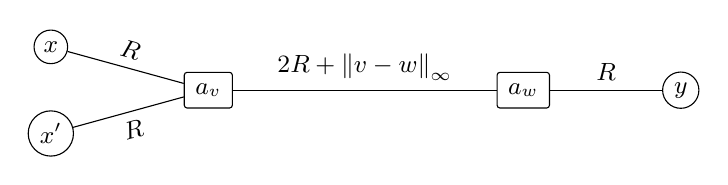
\begin{tikzpicture}[every node/.style={font=\small}]
 \node[circle,draw,inner sep=2pt] (x) at (0,0.55) {$x$};
 \node[circle,draw,inner sep=2pt] (xx) at (0,-0.55) {$x'$};
 \node[draw,rounded corners=1pt,inner sep=4pt] (a) at (2,0) {$a_v$};
 \node[draw,rounded corners=1pt,inner sep=4pt] (b) at (6,0) {$a_w$};
 \node[circle,draw,inner sep=2pt] (y) at (8,0) {$y$};
 \draw (x) -- node[above,sloped] {$R$} (a);
 \draw (xx) -- node[below,sloped] {$R$} (a);
 \draw (a) -- node[above] {$2R+\norm{v-w}_\infty$} (b);
 \draw (b) -- node[above] {$R$} (y);
\end{tikzpicture}
\caption{The added edges when $x,x'$ share label $v$ and $y$ has a different
label $w$.
The source vertices may belong to different graphs. Lines represent weighted
edges between vertices; their interiors are not points of $M_p$. Routes
through anchors can shorten long distances within a source graph.}
\label{fig:anchors}
\end{figure}

\begin{lemma}\label{lem:block-geometry}
The preceding construction has the following properties.
\begin{enumerate}[label=\textup{(\roman*)}]
\item $(M_p,d_p,o)$ is a countably infinite pointed metric space with
separation at least one and diameter at most $B=B_p$. The anchor set $A_p$
is finite and contains $o$. Each source edge has endpoints at $d_p$-distance
at most one.
\item The label map $h:M_p\to\{0,\ldots,D\}^k$ is 1-Lipschitz for the
sup norm. If a source vertex $x$ has color $i$, then $h_i(x)=0$, and
$h(a(x))=h(x)$.
\item For every source vertex $x$ and every anchor $a$,
\[
 d_p(x,a)\ge R=R_p,\qquad d_p(x,a(x))=R.
\]
In particular, $d_p(x,o)\ge R_p=30p$.
\item Every closed $d_p$-ball of radius $2L$ has at most $Q$ points.
For every $t\in M_p$, at most $H$ coordinates of $h(t)$ are strictly
below $D$.
\end{enumerate}
\end{lemma}

\begin{proof}
There are at most $(D+1)^k$ possible labels, so $A_p$ is finite. The disjoint
union of the nonempty finite graphs is countably infinite, and adjoining
finitely many anchors preserves that cardinality. The added edges connect
all vertices. Every edge length is a positive integer: this is clear for
source and attachment edges, and the sup distance between two integer labels
is an integer. For distinct endpoints the lengths of connecting finite paths
therefore form a nonempty subset of the positive integers, which has a least
element. Thus the infimum defining $d_p$ is attained. Symmetry and the
triangle inequality follow from reversal and concatenation of paths, and
distinct points have distance at least one. This also justifies using a
shortest path despite the possible infinite degrees of anchors. A source edge
itself gives distance at most one between its endpoints; for a loop the
distance is zero.

The sup distance between any two labels is at most $D$. Two source vertices
with different anchors can be joined by their two attachment edges and one
anchor edge, with total length at most
\[
 R+(2R+D)+R=4R+D=B.
\]
If their anchors agree, the route through that single anchor has length
$2R$. A source vertex and an anchor have distance at most $3R+D$, and two
anchors have distance at most $2R+D$, with the coincident-anchor cases
shorter. These bounds prove the diameter assertion. Any path from a source
vertex to an anchor must enter the anchor set for the first time along an
attachment edge of length $R$. Hence $d_p(x,a)\ge R$ for every anchor $a$.
The edge from $x$ to $a(x)$ realizes length $R$, proving (iii).

Across a source edge, the distances to a fixed color class differ by at most
one whenever that color is present in the component: append the edge to a
path realizing either distance. Capping at $D$ preserves this bound. If the
color is absent from the component, both coordinates are $D$. Thus adjacent
source labels have sup distance at most one. Labels agree across an
attachment edge, while each anchor edge has length at least the sup distance
between its endpoint labels. Summing these inequalities along any path gives
\[
 \norm{h(u)-h(v)}_\infty\le d_p(u,v).
\]
The own-color coordinate is zero by its definition, and anchor labels were
copied from their assigned vertices. This proves (ii), including paths that
use anchor shortcuts.

Every added edge has length at least $R=3L>2L$. A shortest path of length at
most $2L$ therefore uses only source edges. The closed radius-$2L$ ball about
an anchor is a singleton, and that about a source vertex is contained in its
radius-$2L$ ball in its own source graph. In a $\Delta$-regular multigraph, every vertex
at graph distance at most $s$ is reached by a walk of some length at most
$s$, and there are at most $\Delta^t$ walks of length $t$ from a fixed
vertex. Loops, parallel edges, and repeated vertices may cause several counted
walks to reach the same vertex. Therefore every such metric ball has at most
\[
 \sum_{t=0}^{2L}\Delta^t\le\Delta^{2L+1}=Q
\]
points. The inequality follows from the geometric sum formula and
$\Delta\ge2$.

Finally, if $h_i(x)<D$ at a source vertex, its integer graph distance to a
vertex of color $i$ is at most $D-1$. Witnesses for distinct colors are
distinct vertices, so the number of such coordinates is at most
\[
 \sum_{t=0}^{D-1}\Delta^t\le\Delta^{D+1}=H.
\]
Every anchor copies a source label, giving the same bound at all points of
$M_p$. This proves (iv).
\end{proof}

Part (iii) also gives a direct geometric proof that the wedge in
\Cref{sec:reduction} is unbounded. Each block contains a source vertex,
and the wedge preserves its distance from the common basepoint, which is
at least $R_p=30p$.

The construction has now fixed $M_p$, its finite anchor set, and the entire
graph sequence independently of any operator. The ball bound gives at most
$Q$ nearby successors for any point in any eventual finite support. The
label bound gives a second restriction: if a source vertex $x$ has color
$i$ and $\norm{h(x)-h(t)}_\infty<D$, then $h_i(t)<D$ because $h_i(x)=0$.
For each fixed $t$, proximity of labels therefore permits at most $H$
source colors. Both restrictions hold for every possible support, including
one containing anchors or vertices from several source graphs.

\section{Finite-rank operators and signed measures}\label{sec:operators}

Fix an integer $p\ge1$ and the block $(M_p,d_p,o)$ constructed in
\Cref{lem:block-geometry}, with its anchors $A_p$, label map $h$, and
parameters from \eqref{eq:parameters}. We now begin the proof of
\Cref{thm:blocks}. An operator that approximates the anchors will give a
signed measure at each graph vertex. The measure will have bounded total
variation and a large integral against a bump determined by that vertex's
label. These two estimates are the inputs for the graph argument.

\subsection{A common finite support}

Finite rank does not imply that the range is supported on finitely many
evaluations. The following perturbation supplies such a support while
retaining the bounds needed later.

\begin{lemma}\label{lem:finite-support}
Suppose that a bounded finite-rank linear operator
$T_0:\F(M_p)\to\F(M_p)$ satisfies $\norm{T_0}\le p$ and
\[
 \norm{T_0\delta_a-\delta_a}<\frac12\qquad(a\in A_p).
\]
Then there are a finite set $S\subseteq M_p$ containing $o$ and a bounded
finite-rank linear operator $T:\F(M_p)\to\F(M_p)$ such that
\begin{equation}\label{eq:operator-bounds}
 \begin{gathered}
 T\F(M_p)\subseteq\operatorname{span}\{\delta_j:j\in S\},\qquad
 \norm{T}\le2p,\\
 \norm{T\delta_a-\delta_a}<1\qquad(a\in A_p).
 \end{gathered}
\end{equation}
\end{lemma}

\begin{proof}
If $T_0=0$, take $T=0$ and $S=\{o\}$; the assumed anchor errors already
give the required bounds. Otherwise choose a basis $v_1,\ldots,v_r$ of
the range of $T_0$. The coordinate functionals on this finite-dimensional
range are bounded. Composing them with $T_0$ gives bounded functionals
$\phi_i$ on $\F(M_p)$ such that
\[
 T_0u=\sum_{i=1}^r\phi_i(u)v_i.
\]
Choose $0<\eta<\min\{p,1/(2B)\}$. Finite linear combinations of
evaluations are dense in $\F(M_p)$, so we can choose such combinations
$w_i$ with
\[
 \sum_{i=1}^r\norm{\phi_i}\norm{w_i-v_i}<\eta.
\]
The operator $Tu=\sum_i\phi_i(u)w_i$ then satisfies
$\norm{T-T_0}<\eta$. Let $S$ be the union of $\{o\}$ and the finite
supports of the chosen combinations $w_i$. Its range has the asserted
support, and $\norm{T}\le p+\eta<2p$. Since
$\norm{\delta_a}=d_p(a,o)\le B$, for every $a\in A_p$ we also have
\[
 \norm{T\delta_a-\delta_a}
 \le\norm{T_0\delta_a-\delta_a}+\norm{T-T_0}\norm{\delta_a}
 <\frac12+\eta B<1.\qedhere
\]
\end{proof}

\subsection{Measures detected by label bumps}

For a source vertex $x$, define a function on all of $M_p$ by
\begin{equation}\label{eq:bump}
 b_x(t)=L\left(1-\frac{\norm{h(x)-h(t)}_\infty}{K}\right)_+,
 \qquad s_+=\max\{s,0\}.
\end{equation}
The label map is $1$-Lipschitz by \Cref{lem:block-geometry}. Hence $b_x$
takes values in $[0,L]$, has Lipschitz constant at most $L/K\le1$, and
equals $L$ at the anchor $a(x)$, whose label is $h(x)$. The small
Lipschitz constant will let us compare $T\delta_x$ with the nearby
anchor evaluation even when $\norm{T}$ is as large as $2p$.

For a signed measure $\nu$ on a finite set $S$, write
\[
 |\nu|(E)=\sum_{j\in E}|\nu(\{j\})|\quad(E\subseteq S),
 \qquad \norm{\nu}_{\TV}=|\nu|(S).
\]

\begin{lemma}\label{lem:measure-bounds}
Let $S\subseteq M_p$ be finite and contain $o$, and let
$T:\F(M_p)\to\F(M_p)$ be a bounded linear operator satisfying
\eqref{eq:operator-bounds}. There is a family $(\mu_x)_{x\in M_p}$ of
signed measures on $S$, each of total mass one, such that
\begin{equation}\label{eq:affine-pairing}
 \int g\,d\mu_x=(T\delta_x)(g-g(o))+g(o)
\end{equation}
for every real Lipschitz function $g$ on $M_p$. They satisfy
\begin{equation}\label{eq:tv-bound}
 \norm{\mu_x}_{\TV}\le V=1+4pB\qquad(x\in M_p),
\end{equation}
and, for every source vertex $x$,
\begin{equation}\label{eq:bump-mass}
 \int b_x\,d\mu_x\ge\frac{3L}{4}.
\end{equation}
\end{lemma}

\begin{proof}
For each $x$, express
$T\delta_x=\sum_{j\in S\setminus\{o\}}c_x(j)\delta_j$ and set
\[
 \mu_x(\{j\})=c_x(j)\quad(j\ne o),\qquad
 \mu_x(\{o\})=1-\sum_{j\in S\setminus\{o\}}c_x(j).
\]
The empty sum is zero when $S=\{o\}$. These masses sum to one, and
\[
 \int g\,d\mu_x
 =\sum_{j\in S\setminus\{o\}}c_x(j)\bigl(g(j)-g(o)\bigr)+g(o),
\]
which is \eqref{eq:affine-pairing}.

To estimate the total variation, let $g$ take the sign of
$\mu_x(\{j\})$ at each $j\in S$ and be zero off $S$, using
$\operatorname{sign}(0)=0$. Its values lie in $[-1,1]$, so separation by one gives
$\Lipnorm{g}\le2$. Thus
\[
 \begin{split}
 \norm{\mu_x}_{\TV}
 &=\int g\,d\mu_x\\
 &=(T\delta_x)(g-g(o))+g(o)
 \le2\norm{T\delta_x}+1
 \le1+4pB.
 \end{split}
\]
The last inequality uses $\norm{T}\le2p$ and
$\norm{\delta_x}=d_p(x,o)\le B$. In particular, the estimate includes
the mass at the basepoint.

For a source vertex $x$, \Cref{lem:block-geometry} gives
$d_p(x,a(x))\le R$. The anchor bound in \eqref{eq:operator-bounds}
therefore implies
\[
 \begin{split}
 \norm{T\delta_x-\delta_{a(x)}}
 &\le\norm{T(\delta_x-\delta_{a(x)})}
       +\norm{T\delta_{a(x)}-\delta_{a(x)}}\\
 &\le2pR+1.
 \end{split}
\]
Since $b_x(a(x))=L$, the affine pairing gives
\[
 \begin{split}
 \int b_x\,d\mu_x-L
 &=(T\delta_x-\delta_{a(x)})(b_x-b_x(o))\\
 &\ge-\frac{L}{K}(2pR+1).
 \end{split}
\]
Here $(2pR+1)/K\le1/5<1/4$, because $K=10p(R+1)$ and $p\ge1$.
This proves \eqref{eq:bump-mass}.
\end{proof}

The measures may have coefficients of either sign. Their common total
mass means that $\mu_x-\mu_y$ annihilates constants, so a scalar test
can be centered at $o$ without changing its pairing with this difference.
Signed representations also occur in Lipschitz almost extension;
\cite[Proposition~6 and Remark~7]{Naor21} distinguishes them from the
restrictions imposed by probability measures. Here the total-variation
bound is what permits arbitrary signs in $T$.

\section{Rare matched walks and continuation records}\label{sec:walks}

Fix a finite set $S\subseteq M_p$ containing $o$. Its points will serve
as states, and its labels and metric distances remain fixed throughout
the following argument. The set may be the support obtained from an
operator in \Cref{lem:finite-support}; its points may lie in any of the
graphs or among the anchors. We will select a graph only after $S$ has
been fixed.

Recall the incidence convention from \Cref{sec:blocks}. Each edge
instance has two distinct oriented incidences $e,\bar e$, exchanged
by reversal, including when the edge is a loop. A loop therefore counts
twice toward degree. Write $e:x\to y$ and let $\mathcal D(x)$ be the
set of $\Delta$ outgoing incidences at $x$. A walk is
\emph{nonbacktracking} if it never immediately takes the reverse
incidence of its preceding step.

In the application to \Cref{lem:measure-bounds}, we will compare the
measures at the ends of an incidence $e:x\to y$ using a $1$-Lipschitz
function that agrees with $b_x$ on one subset of $S$ and with $-b_y$ on
another. This section supplies the combinatorial rule for choosing those
subsets from the fixed graph sequence and the labels and distances on $S$.

A graph vertex $x$ and a state $j\in S$ are \emph{compatible} when
\[
 \norm{h(x)-h(j)}_\infty\le K+2L+1=D-4.
\]
A nonbacktracking walk $x_0,e_1,x_1,\ldots,e_t,x_t$ in one graph
$G_m$ is \emph{matched} if there are states $j_0,\ldots,j_t\in S$
such that $(x_s,j_s)$ is compatible for every $s$ and
\[
 d_p(j_{s-1},j_s)\le2L\qquad(1\le s\le t).
\]
Both the states and the source vertices may repeat. For example, a
return along a different parallel edge is allowed; only the reverse
of the preceding incidence is forbidden.

The compatibility threshold allows for a label distance below $K$ where
a bump is positive, one source-edge step of length at most one, and one
state step of length at most $2L$. The inequality $K+2L+1<D$ will also
restrict the possible source colors.

\subsection{A long match is rare}

Each state has at most $Q$ possible successors, by the radius-$2L$
ball bound in \Cref{lem:block-geometry}, while a graph walk encounters
many possible colors. We use this disparity to bound the
fraction of roots from which a long matched walk starts.

\begin{lemma}\label{lem:rare-walks}
For a fixed integer $n\ge1$, let $\beta_m$ be the fraction of vertices
of $G_m$ from which a matched walk of length $n$ starts. Then
\begin{equation}\label{eq:bad-fraction}
 \limsup_{m\to\infty}\beta_m
 \le |S|\frac Hk\left(\frac{\Delta QH}{k}\right)^n.
\end{equation}
Consequently one can choose $n\ge2$ and then $m$ so that
$\beta_m<1/(20V)$.
\end{lemma}

\begin{proof}
For $j\in S$, set
\[
 C_j=\{i:h_i(j)<D\}.
\]
\Cref{lem:block-geometry} gives $|C_j|\le H$. If $x$ has color $i$
and is compatible with $j$, then $h_i(x)=0$ implies
\[
 h_i(j)\le K+2L+1=D-4<D.
\]
Thus the color of $x$ belongs to $C_j$. This is only a necessary
condition for compatibility; it avoids any independence assertion
about the full labels.

Consider the weaker event that a nonbacktracking length-$n$ walk
$x_0,e_1,x_1,\ldots,e_n,x_n$ from the root has states
$j_0,\ldots,j_n\in S$ with $d_p(j_{s-1},j_s)\le2L$ for $1\le s\le n$
and with the color of $x_s$ in $C_{j_s}$ for $0\le s\le n$.
Its occurrence is determined
by the induced colored radius-$n$ ball: every traversed vertex and
edge lies in that ball, including loops and parallel edge instances.
There are only finitely many such rooted types. With $S$ and $n$ fixed,
the sets $C_j$ and the transition relation are fixed, so the event selects
the same finite union of these types for every $m$.
\Cref{lem:local-limit} gives convergence for
every type and therefore for this particular finite union. Its empirical
frequency converges to its probability on the independently colored
$\Delta$-regular tree. The support may have been chosen using the entire
deterministic graph sequence: once fixed, it only selects the types in
the union. No random colors are conditioned on the support.

On the tree there are at most $\Delta^n$ nonbacktracking walks of
length $n$ from the root, each visiting $n+1$ distinct vertices.
For each state $j$, its allowed successors lie in
$S\cap\overline B_{d_p}(j,2L)$, which has at most $Q$ points.
Thus there are at most $|S|Q^n$ allowed state sequences. For a fixed
walk and state sequence, independence of the colors gives probability
at most $(H/k)^{n+1}$ for all required memberships. Repeated states
and overlapping sets $C_j$ do not affect this product, because the
source vertices on the tree are distinct. A union bound gives
\[
 \Delta^n|S|Q^n(H/k)^{n+1}
 =|S|(H/k)(\Delta QH/k)^n.
\]
Every matched walk satisfies the weaker event, proving
\eqref{eq:bad-fraction}. Finally, $k>2\Delta QH$ gives
$\Delta QH/k<1/2$. Choose $n\ge2$ so that the right-hand side of
\eqref{eq:bad-fraction} is less than $1/(40V)$, and then choose $m$
with $\beta_m<1/(20V)$.
\end{proof}

\begin{remark}[Adding roots with non-tree neighborhoods]\label{rem:non-tree-bad-set}
One may enlarge the set counted by $\beta_m$ to include every root whose
induced radius-$(n+1)$ neighborhood is not a tree. For fixed $n$, let
$\gamma_m$ be the fraction of roots with such a neighborhood and
$\widetilde\beta_m$ the enlarged fraction. Then
$\beta_m\le\widetilde\beta_m\le\beta_m+\gamma_m$, while the local limit
gives $\gamma_m\to0$. Thus \eqref{eq:bad-fraction} remains valid with
$\widetilde\beta_m$ in place of $\beta_m$, and the same successive choices
of $n\ge2$ and sufficiently large $m$ give
$\widetilde\beta_m<1/(20V)$.
\end{remark}

\subsection{At most one exceptional direction per state}

Fix $n\ge2$ and one graph $G=G_m$. Call a vertex \emph{bad} if a
matched walk of length $n$ starts there, and \emph{good} otherwise.
The next argument is deterministic. At a good vertex it uses the
absence of long matched walks to select at most one direction for
each state.

A related comparison of nonbacktracking continuation lengths appears in
Ben-David, Childs, Gily\'en, Kretschmer, Podder, and Wang
\cite[\S6.1.2, Algorithm~6.1 and Lemma~6.3]{BenDavidEtAl24}. Their
probabilistic graph algorithm uses such lengths to select parent directions,
and their consistency lemma excludes an incompatible pair of choices by
symmetric length inequalities. Here the
records are deterministic and indexed by support states; the incidence
formulation also includes loops and parallel edges. The argument below is
self-contained.

For a good vertex $x$, an incidence $e\in\mathcal D(x)$, and a
state $j\in S$, let $\mathcal L_x(e,j)$ be the set of positive integer
lengths of matched walks starting through $e$ with initial state $j$.
Define
\[
 r_x(e,j)=\max\bigl(\{0\}\cup\mathcal L_x(e,j)\bigr).
\]
A matched walk of length at least $n$
has a matched prefix of length $n$, so
$\mathcal L_x(e,j)\subseteq\{1,\ldots,n-1\}$. Thus the maximum is
well-defined. The value zero means only that no positive-length walk
exists; it makes no assertion about compatibility of $(x,j)$.

Declare $e$ \emph{exceptional at $(x,j)$} if its record is strictly
greater than every other outgoing record at $(x,j)$. There is at most
one such incidence; if largest records are tied, there is none. At a
bad vertex, declare all outgoing incidences exceptional at every state.
For an incidence $e:x\to y$, set
\[
 E_e=\{j\in S:e\text{ is exceptional at }(x,j)\}.
\]

\begin{lemma}\label{lem:exceptional-directions}
Let $e:x\to y$ be an incidence of $G$ and let $j,j'\in S$ be states.
If $(x,j)$ and $(y,j')$
are compatible and $d_p(j,j')\le2L$, then
$j\in E_e$ or $j'\in E_{\bar e}$.
\end{lemma}

\begin{proof}
If either endpoint is bad, the conclusion follows from the definition.
Suppose both are good, and put
\[
 A_x=\max_{g\in\mathcal D(x)\setminus\{e\}}r_x(g,j),
 \qquad
 A_y=\max_{f\in\mathcal D(y)\setminus\{\bar e\}}r_y(f,j').
\]
The maxima are over nonempty finite sets, since $\Delta\ge4$. If
$A_y>0$, choose a walk
realizing it and prepend $e$, with the state transition $j$ to $j'$.
The old first incidence is not $\bar e$, so the resulting walk is
nonbacktracking and matched. If $A_y=0$, the edge alone, with states
$j,j'$, is a matched walk. The same argument after reversing $e$
therefore gives both inequalities
\begin{equation}\label{eq:record-inequalities}
 r_x(e,j)\ge1+A_y,\qquad r_y(\bar e,j')\ge1+A_x.
\end{equation}
If neither incidence were exceptional, their records would be at
most $A_x$ and $A_y$, respectively. These inequalities would force
\[
 A_x\ge1+A_y\ge2+A_x,
\]
a contradiction.
\end{proof}

The proof uses incidence identities, so it also applies to loops and
parallel edges. It allows repeated states and vertex revisits, and using
the edge by itself covers zero records. The conclusion will let us
prescribe opposite scalar values at the two endpoints: whenever nearby
states could receive opposing nonzero values, at least one of their
prescriptions must be discarded.

\section{Scalar tests and incidence averaging}\label{sec:tests}

Keep the finite state set $S$, the integer $n\ge2$, and the graph
$G=G_m$ from the continuation construction in \Cref{sec:walks}.
For an incidence $e:x\to y$, we will prescribe the bump $b_x$ on
states outside $E_e$ and the negative bump $-b_y$ on states outside
$E_{\bar e}$. The bump bounds handle pairs within one set and cross pairs
at distance at least $2L$. The exceptional-direction lemma handles closer
cross pairs, making the combined prescribed values $1$-Lipschitz.

\begin{lemma}\label{lem:edge-test}
For every incidence $e:x\to y$ of $G$, there is a $1$-Lipschitz
function $f_e:M_p\to[-L,L]$ such that
\[
 f_e(j)=b_x(j)\quad(j\in S\setminus E_e),\qquad
 f_e(j')=-b_y(j')\quad(j'\in S\setminus E_{\bar e}).
\]
\end{lemma}

\begin{proof}
Within either prescription set, the Lipschitz inequality follows from
the bump bound. Across the two sets, the difference between the
prescribed values at $j,j'$ is
$b_x(j)+b_y(j')\le2L$. Thus the inequality holds whenever
$d_p(j,j')\ge2L$.

Suppose $d_p(j,j')<2L$ and $b_x(j)>0$. Then
$\norm{h(x)-h(j)}_\infty<K$. Since $d_p(x,y)\le1$ and $h$ is
$1$-Lipschitz, \Cref{lem:block-geometry} gives
\[
 \begin{split}
 \norm{h(y)-h(j')}_\infty
 &\le\norm{h(y)-h(x)}_\infty
       +\norm{h(x)-h(j)}_\infty
       +\norm{h(j)-h(j')}_\infty\\
 &<1+K+2L.
 \end{split}
\]
The pairs $(x,j)$ and $(y,j')$ are compatible, and their state distance
is at most $2L$. By \Cref{lem:exceptional-directions}, both
prescriptions cannot be present. The same reasoning applies when
$b_y(j')>0$. Hence whenever two states, one from each prescription set,
are less than $2L$ apart, both prescribed values are zero. This proves
the remaining Lipschitz inequalities and, by taking $j=j'$, consistency
on the intersection of the two prescription sets.

Let $P\subseteq S$ be their union and $v:P\to[-L,L]$ the resulting
$1$-Lipschitz data. If $P$ is empty, take $f_e=0$. Otherwise the
classical scalar Lipschitz extension principle \cite{McShane34}
can be realized for these finite data by the following formula,
followed by clipping:
\[
 F(z)=\min_{j\in P}\{v(j)+d_p(z,j)\},\qquad
 f_e(z)=\max\{-L,\min\{L,F(z)\}\}.
\]
For $z\in P$, the Lipschitz inequalities for $v$ give $F(z)=v(z)$.
The triangle inequality gives $F(z)\le F(w)+d_p(z,w)$ and the
same inequality with $z,w$ exchanged. Thus $F$ is $1$-Lipschitz.
Clipping to $[-L,L]$ preserves both the Lipschitz bound and the
prescribed values.
\end{proof}

\subsection{The finite anchor obstruction}

Each test compares the signed measures at the ends of its incidence.
The comparison loses variation only on exceptional states. At a good
vertex each state is exceptional in at most one of the $\Delta$
directions, so averaging these losses will give a bound independent
of the cardinality of $S$.

\begin{proof}[Proof of \Cref{thm:blocks}]
For the chosen integer $p$, \Cref{lem:block-geometry} supplies the
countably infinite block, its separation and diameter bounds, and the
finite anchor set $A_p$. Suppose that a bounded finite-rank operator
$T_0$ of norm at most $p$ has error less than $1/2$ on every anchor.
Choose $T,S$ by \Cref{lem:finite-support} and the measures $\mu_x$
by \Cref{lem:measure-bounds}. With this state set fixed, choose
$n\ge2$ and then $G=G_m$ by \Cref{lem:rare-walks}, so that the
fraction $\beta$ of bad vertices is less than $1/(20V)$. Apply
\Cref{lem:exceptional-directions} and \Cref{lem:edge-test} to these choices.

For an incidence $e:x\to y$, the test prescriptions imply
\begin{align}
 \int f_e\,d(\mu_x-\mu_y)
 &\ge\int b_x\,d\mu_x+\int b_y\,d\mu_y\notag\\
 &\quad-2L\bigl(|\mu_x|(E_e)+|\mu_y|(E_{\bar e})\bigr)\notag\\
 &\ge\frac{3L}{2}
       -2L\bigl(|\mu_x|(E_e)+|\mu_y|(E_{\bar e})\bigr).
       \label{eq:edge-lower}
\end{align}
Indeed, $f_e-b_x$ vanishes on $S\setminus E_e$ and has absolute value
at most $2L$ elsewhere; the same statement holds for $f_e+b_y$ and
$E_{\bar e}$. Integration against the variation measures bounds both
errors, regardless of the signs of the coefficients.

On the other hand, the affine pairing \eqref{eq:affine-pairing} gives
\begin{equation}\label{eq:edge-upper}
 \left|\int f_e\,d(\mu_x-\mu_y)\right|
 =\left|(T(\delta_x-\delta_y))(f_e-f_e(o))\right|
 \le2p,
\end{equation}
because $\norm{T}\le2p$, $\Lipnorm{f_e}\le1$, and
$\norm{\delta_x-\delta_y}=d_p(x,y)\le1$. For a loop, $x=y$ and
the left side is zero.

Choose a uniform vertex $x$ of $G$ and then a uniform incidence
$e\in\mathcal D(x)$. At a good vertex each fixed state occurs in
at most one exceptional set. Consequently
\[
 \frac1\Delta\sum_{e\in\mathcal D(x)}|\mu_x|(E_e)
 \le\frac1\Delta\sum_{j\in S}|\mu_x(\{j\})|
 \le\frac V\Delta.
\]
At a bad vertex the average is at most $V$. Therefore
\begin{equation}\label{eq:average-error}
 \E\bigl[|\mu_x|(E_e)\bigr]\le\frac V\Delta+V\beta<\frac1{10}.
\end{equation}
The $\Delta$-regularity of $G$ makes this sampling uniform on all oriented
incidences.
Reversal preserves that uniform distribution, exchanging the two
incidences of a loop as well. Hence
$\E\bigl[|\mu_y|(E_{\bar e})\bigr]<1/10$ too. Taking expectations in
\eqref{eq:edge-lower} and using \eqref{eq:edge-upper} forces
\[
 2p>\frac{3L}{2}-\frac{4L}{10}
    =\frac{11L}{10}=11p,
\]
a contradiction.

The construction fixed $p$, all constants, the entire graph sequence,
$M_p$, and $A_p$ before $T_0$ was considered. Only after $T_0$ produced
the finite support $S$ were $n$ and then $m$ chosen. Thus the same finite
anchor set defeats every operator in the stated class, proving
\Cref{thm:blocks}.
\end{proof}

\Cref{thm:blocks} now supplies the hypothesis used in \Cref{sec:reduction}.
The wedge construction there therefore proves \Cref{thm:main}, and the
coefficient identification proves \Cref{cor:renorming}.
\Cref{sec:nonlinear} then gives failure of nonlinear approximability for
the same space $\F(M)$.

\begin{remark}[A sufficient criterion for the anchor obstruction]\label{rem:abstract-obstruction}
The preceding proof gives the same finite-anchor obstruction for any data
satisfying the following assumptions. Fix an integer $p\ge1$
and retain the parameter choices
$L,R,K,D,B,V,\Delta,Q,H,k$ of \Cref{sec:blocks}, including
\eqref{eq:parameters}, and the incidence convention of that section.
\begin{enumerate}[label=(\roman*)]
\item $(N,d,o)$ is a countable pointed metric space of separation at
least one and diameter at most $B$, and $A\subseteq N$ is finite
and contains $o$.
\item The $G_m$ are nonempty finite $\Delta$-regular multigraphs with disjoint
vertex sets in $N$ and colors in $\{1,\ldots,k\}$. Edge endpoints
have $d$-distance at most one. For every fixed integer $r\ge0$, the
empirical distributions of their induced rooted radius-$r$ colored
balls converge to the corresponding distribution on the $\Delta$-regular
tree with independent uniform colors, as in \Cref{lem:local-limit}.
\item The map $h:N\to\{0,\ldots,D\}^k$ is $1$-Lipschitz for the sup
norm. Every graph vertex $x$ of color $i$ satisfies $h_i(x)=0$ and
has an anchor $a(x)\in A$ with $h(a(x))=h(x)$ and $d(x,a(x))\le R$.
\item Every closed $d$-ball of radius $2L$ has at most $Q$ points,
and for every $t\in N$ at most $H$ coordinates of $h(t)$ are strictly below $D$.
\end{enumerate}
If these data are fixed before $T_0$, every bounded finite-rank real
linear operator $T_0:\F(N)\to\F(N)$ with $\norm{T_0}\le p$ satisfies
\[
 \max_{a\in A}\norm{T_0\delta_a-\delta_a}\ge\frac12.
\]
Indeed, the support perturbation and signed-measure estimates use only
the stated metric, anchor, and label bounds, while the rare-walk,
continuation, scalar-test, and averaging steps use only those bounds,
the stated graph limit, and the incidence convention.
\end{remark}

\begin{thebibliography}{99}

\bibitem{AACD20}
F.~Albiac, J.~L. Ansorena, M.~C\'uth, and M.~Doucha,
\emph{Lipschitz free $p$-spaces for $0<p<1$},
Israel Journal of Mathematics \textbf{240} (2020), no.~1, 65--98.
\href{https://doi.org/10.1007/s11856-020-2061-5}{doi:10.1007/s11856-020-2061-5}.
\href{https://arxiv.org/abs/1811.01265v2}{Preprint: arXiv:1811.01265v2}.

\bibitem{ArensEells56}
R.~F. Arens and J.~Eells, Jr.,
\emph{On embedding uniform and topological spaces},
Pacific Journal of Mathematics \textbf{6} (1956), no.~3, 397--403.
\href{https://doi.org/10.2140/pjm.1956.6.397}{doi:10.2140/pjm.1956.6.397}.

\bibitem{BenDavidEtAl24}
S.~Ben-David, A.~M. Childs, A.~Gily\'en, W.~Kretschmer, S.~Podder, and D.~Wang,
\emph{Symmetries, graph properties, and quantum speedups},
SIAM Journal on Computing \textbf{53} (2024), no.~6,
FOCS20-368--FOCS20-415.
\href{https://doi.org/10.1137/23M1573975}{doi:10.1137/23M1573975}.

\bibitem{BenjaminiSchramm01}
I.~Benjamini and O.~Schramm,
\emph{Recurrence of distributional limits of finite planar graphs},
Electronic Journal of Probability \textbf{6} (2001), paper no.~23, 1--13.
\href{https://doi.org/10.1214/EJP.v6-96}{doi:10.1214/EJP.v6-96}.

\bibitem{BrudnyiBrudnyi07}
A.~Brudnyi and Yu.~Brudnyi,
\emph{Metric spaces with linear extensions preserving Lipschitz condition},
American Journal of Mathematics \textbf{129} (2007), no.~1, 217--314.
\href{https://doi.org/10.1353/ajm.2007.0000}{doi:10.1353/ajm.2007.0000}.
\href{https://arxiv.org/abs/math/0404304v4}{Preprint: arXiv:math/0404304v4}.

\bibitem{CuthKalenda26}
M.~C\'uth and O.~F.~K. Kalenda,
\emph{Lipschitz-free spaces over uniformly discrete metric spaces are
3-Schur}, preprint (2026), version~1, April~2, 2026.
\href{https://arxiv.org/abs/2604.01875v1}{arXiv:2604.01875v1}.

\bibitem{Dalet15}
A. Dalet,
\emph{Free spaces over some proper metric spaces},
Mediterranean Journal of Mathematics \textbf{12} (2015), 973--986.
\href{https://doi.org/10.1007/s00009-014-0455-5}{doi:10.1007/s00009-014-0455-5}.
\href{https://arxiv.org/abs/1404.3939v3}{Preprint: arXiv:1404.3939v3}.

\bibitem{Friedman04}
J.~Friedman,
\emph{A proof of Alon's second eigenvalue conjecture and related problems},
preprint (2004), version~1, May~5, 2004.
\href{https://arxiv.org/abs/cs/0405020v1}{arXiv:cs/0405020v1}.

\bibitem{Godefroy15}
G.~Godefroy,
\emph{A survey on Lipschitz-free Banach spaces},
Commentationes Mathematicae \textbf{55} (2015), no.~2, 89--118.
\href{https://doi.org/10.14708/cm.v55i2.1104}{doi:10.14708/cm.v55i2.1104}.

\bibitem{GodefroyKalton03}
G.~Godefroy and N.~J. Kalton,
\emph{Lipschitz-free Banach spaces},
Studia Mathematica \textbf{159} (2003), no.~1, 121--141.
\href{https://doi.org/10.4064/sm159-1-6}{doi:10.4064/sm159-1-6}.

\bibitem{GodefroyOzawa14}
G. Godefroy and N. Ozawa,
\emph{Free Banach spaces and the approximation properties},
Proceedings of the American Mathematical Society \textbf{142} (2014),
1681--1687.
\href{https://doi.org/10.1090/S0002-9939-2014-11933-2}{doi:10.1090/S0002-9939-2014-11933-2}.
\href{https://arxiv.org/abs/1201.0847v2}{Preprint: arXiv:1201.0847v2}.

\bibitem{Kalton04}
N.~J.~Kalton,
\emph{Spaces of Lipschitz and H\"older functions and their applications},
Collectanea Mathematica \textbf{55} (2004), no.~2, 171--217.
\href{https://kaltonmemorial.missouri.edu/assets/docs/collect2004.pdf}{Author archive}.

\bibitem{Kalton12}
N.~J. Kalton,
\emph{The uniform structure of Banach spaces},
Mathematische Annalen \textbf{354} (2012), 1247--1288.
\href{https://doi.org/10.1007/s00208-011-0743-3}{doi:10.1007/s00208-011-0743-3}.

\bibitem{McShane34}
E.~J. McShane,
\emph{Extension of range of functions},
Bulletin of the American Mathematical Society \textbf{40} (1934),
no.~12, 837--842.
\href{https://doi.org/10.1090/S0002-9904-1934-05978-0}{doi:10.1090/S0002-9904-1934-05978-0}.

\bibitem{Naor21}
A.~Naor,
\emph{Impossibility of almost extension},
Advances in Mathematics \textbf{384} (2021), article 107761.
\href{https://doi.org/10.1016/j.aim.2021.107761}{doi:10.1016/j.aim.2021.107761}.
\href{https://arxiv.org/abs/2009.11373v2}{Preprint: arXiv:2009.11373v2}.

\bibitem{Smith26}
R.~J. Smith,
\emph{Lipschitz-free spaces and Bossard's reduction argument},
preprint (2026), version~4, February~23, 2026.
\href{https://arxiv.org/abs/2509.00722v4}{arXiv:2509.00722v4}.

\end{thebibliography}

\end{document}
